%!TEX root = ../../PhD_thesis__Edouard_Leurent.tex
\graphicspath{{2-Chapters/6-Chapter/}}

\chapter{Complements on \Cref{chapter:6}}

\paragraph{Outline}
We provide proofs for every claimed result in \Cref{sec:kl-olop-proofs}.
We look into the time and memory complexity and propose efficient implementations of \OLOP and \KLOLOP in \Cref{sec:kl-olop-time}, and of \GBOPD and \GBOP in \Cref{sec:gbop-implementation}.

\section{Proofs}
\label{sec:kl-olop-proofs}

\subsection{Proof of \Cref{lemma:expected-regret}}
\label{sec:proof-lem-expected-regret}
\begin{proof}
	The proof is identical to that of Lemma 4 in \citep{Bubeck2010}.
	
	Since $\arg \max _{a \in \cA} T_{a}(M)$, and $\sum_{a \in \cA} T_{a}(M)=M,$ we have $T_{a(n)}(M) \geq M / K$, and thus:
	\begin{equation*}
	\frac{M}{K}(V-V(a(n))) \leq(V-V(a(n))) T_{a(n)}(M) \leq \sum_{m=1}^{M} V-V\left(a^{m}\right)
	\end{equation*}
	Hence, we have, $r_{n} \leq \frac{K}{M} \sum_{m=1}^{M} V-V\left(a^{m}\right)$. Now remark that, for any sequence of actions $a\in \cA^L$, we have either:
	\begin{itemize}
		\item $a_{1 : H} \in \mathcal{I}_{H} ;$ which implies $V-V(a) \leq \frac{2 \gamma^{H+1}}{1-\gamma}$
		\item or there exists $1\leq h \leq H$ such that $a_{1:h} \in \mathcal{J}_h$; which implies $V-V(a) \leq V-V\left(a_{1 : h-1}\right)+\frac{\gamma^{h}}{1-\gamma} \leq \frac{3 \gamma^{h}}{1-\gamma}$.
	\end{itemize}
	Thus we can write:
	\begin{equation*}
	\begin{aligned} \sum_{m=1}^{M}\left(V-V\left(a^{m}\right)\right) &=\sum_{m=1}^{M}\left(V-V\left(a^{m}\right)\right)\left(\mathbbm{1}\left\{a^{m} \in \mathcal{I}_{H}\right\}+\mathbbm{1}\left\{\exists 1 \leq h \leq H : a_{1 : h}^{m} \in \mathcal{J}_{h}\right\}\right) \\ & \leq \frac{2 \gamma^{H+1}}{1-\gamma} M+3 \sum_{h=1}^{H} \sum_{a \in \mathcal{J}_{h}} \frac{\gamma^{h}}{1-\gamma} T_{a}(M) \end{aligned}
	\end{equation*}
	
\end{proof}

\subsection{Proof of \Cref{lemma:size_Ph}}
\label{sec:proof-size_Ph}
\begin{proof}
	The event $\tau^a_{h,h'}=1$ implies $a^{m+1}\in a A^*$ and \eqref{eq:sampled-enough}. This implies by \Cref{lemma:sub-optimal-pull} that either \eqref{eq:cond-ukl}, \eqref{eq:cond-lkl} or \eqref{eq:cond-dkl} is satisfied. Now by \Cref{lemma:ci-length} this implies that either \eqref{eq:cond-ukl} is true or \eqref{eq:cond-lkl} is true or \eqref{eq:sampled-enough-h} is false. We now prove that if \eqref{eq:P-min-size} is not satisfied then \eqref{eq:sampled-enough} is true, which clearly ends the proof.
	This follows from: For any $0 \leq t \leq h'$:
	
	\begin{align*}
	T_{a_{1:t}}(m) &= \sum_{b\in a_{1:t}A^{h-t}} T_b(m) \geq \sum_{b\in \mathcal{P}^{a_{1:t}}_{h,h'}} T_b(m) \\
	&\geq \left(\gamma^{2(t-h')}\right) \left(2f(m)(h+1)^2\gamma^{2(h'-h-1)}\right)\\
	&= 2f(m)(h+1)^2\gamma^{2(t-h-1)}\,.\qquad\qquad
	\end{align*}
	%\
\end{proof}

\subsection{Proof of \Cref{lemma:expected-P-size}}
\label{sec:proof-expected_P_size}
\begin{proof}
	The proof is identical to that of Lemma 9 in \citep{Bubeck2010}.
	
	\noindent
	Let $h'\geq 1$ and $0 \leq s \leq h'$. We introduce the following random variables:
	\begin{equation*}
	m_{s}^{a}=\min \left(M, \min \left\{m \geq 0 :\left|\mathcal{P}_{h, h^{\prime}}^{a}(m)\right| \geq \gamma^{2\left(s-h^{\prime}\right)}\right\}\right).
	\end{equation*}
	We will prove recursively that,
	\begin{equation}
	\label{eq:toprove}
	\left|\mathcal{P}_{h, h^{\prime}}^{\emptyset}(m)\right| \leq \sum_{t=0}^{s} \gamma^{2\left(t-h^{\prime}\right)}\left|\mathcal{I}_{t}\right|+\sum_{a \in \mathcal{I}_{s}}\left|\mathcal{P}_{h, h^{\prime}}^{a} \setminus \cup_{t=0}^{s} \mathcal{P}_{h, h^{\prime}}^{a_{1:t}}\left(m_{t}^{a_{1:t}}\right)\right|
	\end{equation}
	The result is true for $s = 0$ since $\mathcal{I}_0 = \{\emptyset\}$ and by definition of $m^\emptyset_0$,
	\begin{equation*}
	\left|\mathcal{P}_{h, h^{\prime}}^{\emptyset}(m)\right| \leq \gamma^{-2 h^{\prime}}+\left|\mathcal{P}_{h, h^{\prime}}^{\emptyset}(m) \setminus \mathcal{P}_{h, h^{\prime}}^{\emptyset}\left(m_{0}^{\emptyset}\right)\right|
	\end{equation*}
	Now let us assume that the result is true for $s<h'$. We have:
	\begin{align*}
	\sum_{a \in \mathcal{I}_{s}}\left|\mathcal{P}_{h, h^{\prime}}^{a}(m) \setminus \cup_{h, h^{\prime}}^{a_{1 : t}}\left(m_{t}^{a_{1 : t}}\right)\right|&=\sum_{a \in \mathcal{I}_{s+1}}\left|\mathcal{P}_{h, h^{\prime}}^{a}(m) \setminus \cup_{t=0}^{s} \mathcal{P}_{h, h^{\prime}}^{a_{1 : t}}\left(m_{t}^{a_{1 : t}}\right)\right|\\
	&\leq \sum_{a \in \mathcal{I}_{s+1}} \gamma^{2\left(s+1-h^{\prime}\right)}+\left|\mathcal{P}_{h, h^{\prime}}^{a}(m) \setminus \cup_{t=0}^{s+1} \mathcal{P}_{h, h^{\prime}}^{a_{1 : t}}\left(m_{t}^{a_{1 : t}}\right)\right|\\
	&= \gamma^{2\left(s+1-h^{\prime}\right)}\left|\mathcal{I}_{s+1}\right|+\sum_{a \in \mathcal{I}_{s+1}}\left|\mathcal{P}_{h, h^{\prime}}^{a}(m) \setminus \cup_{t=0}^{s+1} \mathcal{P}_{h, h^{\prime}}^{a_{1 ; t}}\left(m_{t}^{a_{1 : t}}\right)\right|
	\end{align*}
	which ends the proof of \eqref{eq:toprove}. Thus we proved (by taking $s=h'$ and $m=M$):
	\begin{equation*}
	\begin{aligned}\left|\mathcal{P}_{h, h^{\prime}}^{\emptyset}(M)\right| & \leq \sum_{t=0}^{h^{\prime}} \gamma^{2\left(t-h^{\prime}\right)}\left|\mathcal{I}_{t}\right|+\sum_{a \in \mathcal{I}_{h^{\prime}}}\left|\mathcal{P}_{h, h^{\prime}}^{a}(M) \setminus \cup_{t=0}^{s+1} \mathcal{P}_{h, h^{\prime}}^{a_{1 : t}}\left(m_{t}^{a_{1 : t}}\right)\right.\\ &=\sum_{t=0}^{h^{\prime}} \gamma^{2\left(t-h^{\prime}\right)}\left|\mathcal{I}_{t}\right|+\sum_{a \in \mathcal{J}_{h}}\left|\mathcal{P}_{h, h^{\prime}}^{a}(M) \setminus \cup_{h, h^{\prime}}^{a_{1 : t}}\left(m_{t}^{a_{1 : t}}\right)\right| \end{aligned}
	\end{equation*}
	
	Now, for any $a\in \mathcal{J}_h$, let $\tilde{m} = \max_{0\leq t\leq h'} m_t^{a_{1:t}}$. Note that for $m\geq \tilde{m}$, equation \eqref{eq:P-min-size} is not satisfied. Thus we have
	\begin{equation*}
	\begin{aligned}
	\left|\mathcal{P}_{h, h^{\prime}}^{a} \setminus \cup_{h, h^{\prime}}^{s+1} \mathcal{P}_{h, h^{\prime}}^{a_{1 : t}}\left(m_{t}^{a_{1 : t}}\right)\right|=&\sum_{m=\tilde{m}}^{M-1} \tau_{h, h^{\prime}}^{a}(m+1)=\sum_{m=0}^{M-1} \tau_{h, h^{\prime}}^{a}(m+1) \mathbbm{1}\{\eqref{eq:P-min-size} \text { is not satisfied }\} \\ & \leq \sum_{m=0}^{M-1} \tau_{h, h^{\prime}}^{a}(m+1) \mathbbm{1}\{\eqref{eq:cond-ukl} \text { or }\eqref{eq:cond-lkl}\} \end{aligned}
	\end{equation*}
	where the last inequality results from \Cref{lemma:size_Ph}. Hence, we proved:
	
	\begin{equation*}
	\left|\mathcal{P}_{h, h^{\prime}}^{\emptyset}\right| \leq \sum_{t=0}^{h^{\prime}} \gamma^{2\left(t-h^{\prime}\right)}\left|\mathcal{I}_{t}\right|+\sum_{m=0}^{M-1} \sum_{a \in \mathcal{J}_{h}} \mathbbm{1}\{\eqref{eq:cond-ukl}\text{ or }\eqref{eq:cond-lkl}\}
	\end{equation*}
	
	Taking the expectation and applying \Cref{lemma:boundary-crossing-prob} yield the claimed bound for $h'\geq 1$.
	
	Now for $h' = 0$ we need a modified version of \Cref{lemma:size_Ph}. Indeed in this case one can directly prove that $\tau_{h,0}^a(m+1)=1$ implies that either equation \eqref{eq:cond-ukl} or \eqref{eq:cond-lkl} is satisfied (this follows from the fact that $\tau_{h,0}^a(m+1)=1$ always imply that \eqref{eq:sampled-enough-h} is true for $h'= 0$). Thus we obtain:
	\begin{equation*}
	\left|\mathcal{P}_{h, h^{\prime}}^{\emptyset}\right|=\sum_{m=0}^{M-1} \sum_{a \in \mathcal{J}_{h}} \tau_{h, 0}^{a}(m+1) \leq \sum_{m=0}^{M-1} \sum_{a \in \mathcal{J}_{h}} \mathbbm{1}\{\eqref{eq:cond-ukl}\text{ or }\eqref{eq:cond-lkl}\}
	\end{equation*}
	Taking the expectation and applying \Cref{lemma:boundary-crossing-prob} yield the claimed bound for $h' = 0$ and ends the proof.
	
\end{proof}

\subsection{Proof of \Cref{lemma:expected-plays-count}}
\label{sec:proof-expected-plays-count}
\begin{proof}
	The proof is identical to that of Lemma 10 in \citep{Bubeck2010}:
	\begin{align*}
	\sum_{a \in \mathcal{J}_{h}} T_{a}(M) = {} & \sum_{a \in \mathcal{J}_{h} \backslash \mathcal{P}_{h, h-1}^{\emptyset}} T_{a}(M)+\sum_{h^{\prime}=1}^{h-1} \sum_{a \in \mathcal{P}_{h, h^{\prime}}^{\emptyset} \setminus \mathcal{P}_{h, h^{\prime}-1}^{\emptyset}} T_{a}(M)+\sum_{a \in \mathcal{P}_{h, 0}^{\emptyset}} T_{a}(M)\\
	\leq {} & 2f(m)(h+1)^{2} \gamma^{2(h-2-h)}\left|\mathcal{J}_{h}\right| \\
	 &+ \sum_{h^{\prime}=1}^{h-1} 2f(m)(h+1)^{2} \gamma^{2\left(h^{\prime}-2-h\right)} \log M\left|\mathcal{P}_{h, h^{\prime}}^{\emptyset}\right|+M\left|\mathcal{P}_{h, 0}^{\emptyset}\right|\\
	= {} &\tilde{\cO}\left(\left(\kappa^{\prime}\right)^{h}+\gamma^{-2 h} \sum_{h^{\prime}=1}^{h-1} \gamma^{2 h^{\prime}}\left|\mathcal{P}_{h, h^{\prime}}^{\emptyset}\right|+M\left|\mathcal{P}_{h, 0}^{\emptyset}\right|\right)
	\end{align*}
	Taking the expectation and applying the bound of \Cref{lemma:expected-P-size} give the claimed bound.
	
\end{proof}


%\section{Proof of \GBOP results}
%\label{sec:gbop-proofs}

\subsection{Proof of \Cref{lem:properties-b-tree}}
\label{sec:proof-properties-b-tree}
\begin{proof}
The tightening property is directly obtained by definition of monotonicity.
Let us show the preservation of monotonicity. Let $U$ a monotonic upper-bound, $a\in \cA^h$. Then, for any $b\in \cA$:
\begin{align*}
U(ab) \geq B(U)(ab) \implies 
r(ab) + \gamma U(ab) \geq r(ab) + \gamma B(U)(ab).
\end{align*}
Thus, my taking the $\max$ on $b$,
$
B(U)(a) \geq B^2(U)(a).
$
The same can be obtained for a lower-bound $L$.

The finite time convergence can be obtained by recursion from the leaves to the root, by noticing that if the value of a set of siblings $aA$ is invariant by $B$, then the value of their parent $a$ is invariant by $B^2$.
\end{proof}

\subsection{Proof of \Cref{lem:properties-b-graph}}
\label{sec:proof-properties-b-graph}
\begin{proof}
The proof of tightening and monotonicity preservation is the same as that of \Cref{lem:properties-b-tree}.
The contraction property is standard for the Bellman Operator, see \eg Puterman M., Markov Decision Processes: Discrete Stochastic Dynamic Programming (2005).
\end{proof}

\subsection{Proof of \Cref{lem:sequence-values}}
\label{sec:proof-sequence-values}
\begin{proof}
By definition, for $a\in\cA^h$,
\begin{align*}
V(a) &= \sup_{b\in a\cA^\infty} \sum_{t=1}^\infty \discount^t\mu(b_{1:t}) \\
     &= \sum_{t=1}^h \discount^t\mu(a_{1:t})  \sup_{b\in a\cA^\infty} \sum_{t=h+1}^\infty \discount^t\mu(b_{1:t}) \\
     &= G(s_1,a) \discount^h \sup_{b\in \cA^\infty} \sum_{t=1}^\infty \discount^t\mu(b_{1:t}\text{ starting from $s(a)$}) \\
     &= G(s_1,a) \discount^h V(s(a))
\end{align*}
\end{proof}

\subsection{Proof of \Cref{thm:regret-opd}}
\label{sec:proof-regret-opd}
We recall the main steps of the proof of \citet{Hren2008}.\\

\begin{enumerate}
	\item The recommendation $a_n$ has a maximal depth $d_n$ in the tree, and its gap $\regret = V^\star - V({a_{n,1}})$ is bounded by $\regret \leq \frac{\gamma^{d_n}}{1-\gamma}$. We need to relate $d_n$ to $n$.
	
	\item Each expanded node belongs to $\Tau^\infty = \bigcup_{h\geq 0} \Tau_h^\infty$, where $$\Tau_h^\infty = \left\{a\in \cA^h: V^\star-V(a) \leq \frac{\gamma^h}{1-\gamma}\right\}.$$ Introduce the difficulty measure $\kappa$ such that $|\Tau_h^\infty| = \cO(\kappa^h)$ (the smallest).
	
	\item In the worst case, expanded nodes fully fill the depths of $\Tau^\infty$ up to $d_n$: $n = \sum_{d=1}^{d_n} n_d \leq  C\sum_{d=1}^{d_n} \kappa^d = \begin{cases}
	\cO(d_n) &\text{if $\kappa=1$}\\
	\cO(\kappa^{d_n}) &\text{else.}
	\end{cases}$\\
	Hence $\regret = \begin{cases}
	\cO(\gamma^n) &\text{if $\kappa=1$}\\
	\cO(\gamma^{\frac{\log n}{\log \kappa}}) = \cO(n^{-\frac{\log 1/\gamma}{\log \kappa}}) &\text{else.}
	\end{cases}$
\end{enumerate}

\subsection{Proof of \Cref{lem:shrink}}
\label{sec:proof-shrink}
\begin{proof}
Let $L_2\leq L_1\leq V\leq U_1\leq U_2$, then $\Tau_h^\infty(L_1,U_1) \subset \Tau_h^\infty(L_2,U_2),$ which implies $$|\Tau_h^\infty(L_1,U_1)|^{1/h} \leq |\Tau_h^\infty(L_2,U_2)|^{1/h}$$ and the claimed result in the limit $h\rightarrow\infty$.
\end{proof}

\subsection{Proof of \Cref{thm:regret-bound-U}}
\label{sec:proof-regret-bound-U}
In this proof, we temporarily assume that $U=B(U)$ and $L=B(L)$. We follow the same steps as in the proof of the regret of \OPD.

\begin{remark}
\begin{leftbar}[remarkbar]
It no longer holds that $a_n$ must be of maximal depth $d_n$.  This is due to the fact the exploration bonus $\gamma^h U(a)$ is not depth-wise constant: consider two nodes $a,b$ at the same depth with $R(a) > R(b)$. In \OPD, both get the same bonus $\gamma^h/(1-\gamma)$, and the node $a$ is expanded first. But with the local bonus, $b$ could be expanded in priority rather than $a$, if its own bonus is sufficiently higher than that of $a$, precisely if $R(a)+\gamma^h U(a) < R(b)+\gamma^h U(b)$. For instance, $U(a)=0$ when $a$ is known to be a terminal state while $b$ can lead to future rewards. If after expanding and exploring the subtree of $b$ we find out that $V(b) = 0$, we still return the recommendation $a$, which is of non-maximal depth.
\end{leftbar}
\end{remark}

The regret bound still holds, however. First, notice that:
\begin{lemma}[Expansion]
\begin{leftbar}[lemmabar]
\label{lem:expansion-bound-U}
Whenever a node $a$ of depth $h$ is expanded by the optimistic algorithm, its first action $a_1$ enjoys a simple regret $V(a^\star)-V(a_1) \leq \gamma^h(U(a)-L(a))$. 
\end{leftbar}
\end{lemma}
\begin{proof}
Let $t$ be the time of expansion of $a$, it holds that $\overline{U}_t(b) \leq \overline{U}_t(a)$ for all $b\in \ext{\Tau}_t$, in particular those in a branch starting by an optimal action $a^\star$. Since $U=B(U)$ and $L=B(L)$, we also have $\overline{U}_t(a^\star) = \max_{b\in a^\star A^*} \overline{U}_t(b) \leq \overline{U}_t(a)$, and $\overline{L}_t(a_1) = \max{b\in a_1 A^*} \overline{L}_t(b) \geq  \overline{L}_t(a)$. Thus, $V(a^\star)-V(a_1) \leq \overline{U}_t(a^\star) - \overline{L}_t(a_1) \leq \overline{U}_t(a) - \overline{L}_t(a) = \gamma^h(U(a)-L(a))$.
\end{proof}
 
\begin{lemma}[Recommendation]
\begin{leftbar}[lemmabar]
\label{lem:recommendation-bound-U}
The recommended action $a_n$ has a simple regret $\regret \leq \frac{\gamma^{d_n}}{1-\gamma}$, where $d_n$ is the maximal depth of $\Tau_n$.
\end{leftbar}
\end{lemma}
\begin{proof}
Let $i$ a node of maximal depth $d_n$, and consider the recommended node $a_n$ at time $n$, of depth $d$. In particular, $\overline{L}_n(a_n) \geq \overline{L}_n(i)$, and since $(\overline{L}_t)_t$ is non-decreasing we also have $\overline{L}_n(i) \geq \overline{L}_t(i)$. At the time $t$ when $i$ is expanded, we have $\overline{U}_t(a_n) \leq \overline{U}_t(i)$, and since $(\overline{U}_t)_t$ is non-increasing we also have $\overline{U}_n(a_n) \leq \overline{U}_t(a_n)$. We can conclude with \Cref{lem:expansion-bound-U} applied to $a_n$: $\regret \leq \gamma^d(U(a_n)-L(a_n) = \overline{U}_n(a_n) - \overline{L}_n(a_n)  \leq \overline{U}_t(a_n) - \overline{L}_n(i) \leq \overline{U}_t(i) - \overline{L}_t(i) = \gamma^{d_n}(U(i) - L(i)$, which yields the claimed bound since $U(i) - L(i) \leq V_{\max}-0$.
\end{proof}

\begin{lemma}[Near-optimal nodes]
\begin{leftbar}[lemmabar]
\label{lem:near-optimal-nodes-U}
Every node expanded by \eqref{eq:sampling_rule} is in $$\Tau^\infty(L,U) = \bigcup_{h\geq 0} \Tau^\infty_h(L,U).$$
\end{leftbar}
\end{lemma}
\begin{proof}
Let $a$ be a node of depth $h$ expanded at round $n$, then $\overline{U}_n(a) \geq \overline{U}_n(b)$ for all $b\in\ext{\Tau}_n$. Thus, since $U = B(U)$, we have $\overline{U}(a) = \overline{B(U)}(\emptyset) = B(U)(s_1) \geq V(s_1) = V^\star$. Thus, $V^\star - V(a) \leq \overline{U}(a) - \overline{L}(a) = \gamma^h(U(a) - L(a))$.
\end{proof}

Finally, we can move on to the proof of \Cref{thm:regret-bound-U}.
Let $n_d$ be the number of expanded nodes of depth $d$, by \Cref{lem:near-optimal-nodes-U} we have $n_d \leq |\Tau^\infty_d(L,U)| \leq C\kappa(L,U)^d$. Thus, 
\[n = \sum_{d=1}^{d_n} n_d \leq C\sum_{d=0}^{d_n} \kappa(L,U)^d = C\frac{\kappa(L,U)^{d_n+1}-1}{\kappa(L,U)-1}\]
Hence, $d_n \geq C'\frac{\log n}{\log\kappa(L,U)},$ which along with \Cref{lem:expansion-bound-U} gives the claimed bound.

Note that if $L,\,U$ are monotonic bounds that do not verify $L = B(L)$ and $U=B(U)$, then planning with $B(L),B(U)$ instead will yield the proved bound with a branching factor $\kappa(B(L),B(U))$, and since $L\leq B(L)\leq V\leq B(U)\leq U$ we have $\kappa(B(L),B(U)) \leq \kappa(L,U)$, which still gives \begin{align*}
\regret = \cO\left(n^{-\frac{\log 1/\gamma}{\log \kappa(L,U)}}\right);
\end{align*}

%\section{Proof of \Cref{prop:b-eq-mb}}

%\begin{proof}
%	Let $U$ equivalent to $\cU$, and $a\in T_n$.
%	If $a\in\ext{T_n}$, then necessarily $s(a)\in\ext{\cG_n}$, and both are unchanged by $B_n$ and $\cB_n$ respectively.
%	If $a\in\inte{T_n}$, then necessarily $s(a)\in\int{\cG_n}$. There exist a'
%\end{proof}

%\section{Proof of \Cref{lem:properties-mb}}
%\begin{proof}
%Let $U_1, U_2\in \Real^\Tau_n, a\in\Tau_n$,
%\begin{align*}
%    (M_n^+ U_1 - M_n^+ U_2)(a) &= \min_{a'\in N_n(a)} U_1(a') - \min_{a'\in N_n(a)} U_2(a') \\
%    &= \min_{a'\in N_n(a)} U_1(a') - U_2(a^-) \\
%    &\leq U_1(a^-) - U_2(a^-) \\
%    &\leq \|U_1 - U_2\|_\infty
%\end{align*}
%where $a^-\in \argmin_{a'\in N_n(a)} U_2(a')$. 
%Hence, $\|M_n^+ U_1 - M_n^+ U_2\|_\infty \leq \|U_1 - U_2\|_\infty$
%\end{proof}
%
%\section{Proof of \Cref{prop:pruning}}
%
%\begin{proof}
%Assume $h(a_2) \geq h(a_1)$.
%\begin{align*}
%    V(a_1) - V(a_2) &= R(a_1)- R(a_2) + \underbrace{\left(\gamma^{h(a_1)} - \gamma^{h(a_2)}\right)}_{\geq 0}V(s) \\
%    &\leq R(a_1)- R(a_2) + \left(\gamma^{h(a_1)} - \gamma^{h(a_2)}\right)U(s)\\
%    &= \overline{U}(a_1) - \overline{U}(a_2)
%\end{align*}
%Hence, if this last term is negative, then $V(a_1) - V(a_2)$ is as well.
%\end{proof}

\subsection{Proof of \Cref{lem:equivalence}}
\label{sec:proof-equivalence}
\begin{proof}	
We first show that if $U$ is equivalent to $\cU$, meaning that for any sequence $a\in T(\cG_n)$ we have $U(a) = \cU(s(a))$, then $B_n(U)$ is equivalent to $\cB_n(\cU)$.

By definition of $T(\cG_n)$, any sequence of action $a\in T(\cG_n)$ corresponds to a path $s_1, a_1,\dots,$ $s_{h}, a_{h}, s_{h+1}$ in $\cG_n$. If $a\in\ext{T(\cG_n)}$, then necessarily $s(a)\in\ext{\cG_n}$, and both are unchanged by $B_n$ and $\cB_n$ respectively. Conversely, if $a\in\inte{T}(\cG_n)$, then $s(a)\in\inte{\cG_n}$ by construction. Thus, 
\begin{align*}
B_n(U)(a) &= \max_{b\in \cA} r(s(a), b) + \gamma U({ab}) &\\
&= \max_{b\in \cA} r(s(a), b) + \gamma \cU(s({ab})) &\text{ (by assumption)} \\
&= \max_{b\in \cA} r(s(a), b) + \gamma \cU(P(s({a}),b))\\
&= \cB_n(\cU_n)(s(a)).
\end{align*}

By induction, for any $k>0$ $B_n^k(U)$ is equivalent to $\cB_n^k(\cU)$, and at the limit $k\rightarrow\infty$ it comes that $U_n$ is equivalent to $\cU_n$. The same result can be shown similarly for $L_n$ and $\cL_n$.
\end{proof}

\subsection{Proof of \Cref{lem:expansion-bound}}
\label{sec:proof-expansion-bound}
We start by showing a preliminary lemma.
\begin{lemma}[Bounds of sequence values]
	\begin{leftbar}[lemmabar]
	\label{lem:bounds}
	The bounds $(\overline{L}_n, \overline{U}_n)$ on the value of sequences of actions verify are respectively non-decreasing and non-increasing with respect to $n$, and verify: for all $a\in \cA^*$, $\overline{U_n}(a) = \max_{a'\in a A^\infty} \overline{U}(a')$.
	\end{leftbar}
\end{lemma}
\begin{proof}
	The second property can be easily shown by induction using the fact that $U_n$ and $L_n$ are fixed-points of $B_n$ by definition. Applying this equation at each depth $h$ gives the result. From this observation, we can deduce that $\overline{L}_n$ is increasing with $n$. Indeed, since when $T(\cG_n)$ is expanded with additional nodes compared to $T(\cG_{n-1})$, the leaves $a$ of $T(\cG_{n-1})$ with previous value $L_{n-1}(a)=0$ are updated to $L_n(a) = \max_b r(s(a), b) \geq 0 = L_{n-1}(a)$, and this increase at the leaves is then propagated through $\max_{a'\in a A^\infty}$ to any internal node $a$. Thus, $L_n$ is non-decreasing and likewise, $U_n$ is non-increasing with respect to $n$. The same is obtained directly of the bounds on sequence values $(\overline{L}_n, \overline{U}_n)$.
\end{proof}

Which enables us to proceed to the proof of \Cref{lem:expansion-bound}.
\begin{proof}
	Let $t$ be the time of expansion of $a$, it holds that $\overline{U}_t(b) \leq \overline{U}_t(a)$ for all $b\in T(\cG_n)$. In particular for $b$ in a branch starting by an optimal action $a^\star$ $\overline{U}_t(a) \geq \max_{b\in a^\star A^*}  \overline{U}_t(b) = \overline{U}_t(a^\star)$. Thus, $V(a^\star)-V(a) \leq \overline{U}_t(a^\star) - \overline{L}_t(a) \leq \overline{U}_t(a) - \overline{L}_t(a) = \gamma^h(U_t(a)-L_t(a))$.
\end{proof}

\subsection{Proof of \Cref{lem:recommendation-bound}}
\label{sec:proof-recommendation-bound}
\begin{proof}
	Let $i$ an expanded node of maximal depth $d_n\in\Real\cup\{\infty\}$, and consider the recommended node $a_n$ at time $n$, of depth $d\in\Real\cup\{\infty\}$. In particular, $\overline{L}_n(a_n) \geq \overline{L}_n(i)$, and since $(\overline{L}_t)_t$ is non-decreasing we also have $\overline{L}_n(i) \geq \overline{L}_t(i)$. At the time $t$ when $i$ is expanded, we have $\overline{U}_t(a_n) \leq \overline{U}_t(i)$, and since $(\overline{U}_t)_t$ is non-increasing we also have $\overline{U}_n(a_n) \leq \overline{U}_t(a_n)$. We can conclude with \Cref{lem:expansion-bound} applied to $a_n$: $\regret \leq V^\star - V(a_n) \leq  \gamma^d(U(a_n)-L(a_n) = \overline{U}_n(a_n) - \overline{L}_n(a_n)  \leq \overline{U}_t(a_n) - \overline{L}_n(i) \leq \overline{U}_t(i) - \overline{L}_t(i) = \gamma^{d_n}(U_t(i) - L_t(i)$, which yields the claimed bound since $U(i) - L(i) \leq V_{\max}-0$.
\end{proof}


\subsection{Proof of \Cref{thm:regret-gbop}}
\label{sec:proof-regret-gbop}
\begin{proof}
Let $\kappa'>\kappa_\infty$. Since $\kappa(L_n,U_n)\rightarrow\kappa_\infty$, there exists $n_0\in\Natural$ such that for all $n\geq n_0$, $\kappa(L_n,U_n) \leq \kappa'$.
By \Cref{lem:expansion-bound}, at each iteration $n$ the expanded node must belong to $\Tau^\infty(L_n,U_n)$.
Let $n\geq n_0$, and define $d_0 = \min\{d\in\Natural: \exists t \in[n_0,n], b_t\in \cA^d \}$. By definition, for all $d\geq d_0$, any expanded node of depth $d$ was expanded at a time $t\geq n_0$, and thus $b_t\in\Tau^\infty_t \subset\Tau^\infty_{n_0}$. We denote $n_d$ the number of expanded nodes of depth $d$. If $d_n=\infty$, then $\regret = 0$ and the bound holds. Else, we obtain
\[
n = \sum_{d=0}^{d_0-1}n_d + \sum_{d=d_0}^{d_n} n_d \leq  C_0 + C_1\sum_{d=d_0}^{d_n} (\kappa')^d \leq C_0 + C_1' (\kappa')^{d_n}
\]
And since $\regret \leq \frac{\gamma^{d_n}}{1-\gamma}$ by \Cref{lem:recommendation-bound}, we obtain the claimed bound.

Moreover, given a history of observed transitions up to iteration $n$, the bounds $U_n, L_n$ obtained from \eqref{eq:gbop-t-bounds} on the unrolled tree $T(\cG_n)$ are tighter than those of \eqref{eq:opd-bounds} since $T_n\subset T(\cG_n)$, which implies by \Cref{lem:shrink} that $\kappa(L_n, U_n) \leq \kappa$. We obtain $\kappa_\infty \leq \kappa$ at the limit. 
\end{proof}

\subsection{Proof of \Cref{prop:illustrative-example}}
\label{sec:proof-illustrative-example}
The \Cref{fig:mdp-tree} shows the planning tree corresponding to the MDP $\cM$. Whenever the action $a_1$ is taken \hlg{(in green)} the resulting subtree is represented by a leaf node $s^\star$ of value $V^\star = \frac{r^\star}{1-\gamma}$. When, in contrast, we take a sequence of actions among $a_2\dots a_K$ \hlo{(in orange)}, we stay in the state $s^+$ and denote $V_h$ the corresponding value at depth $h$.

\begin{figure}
    \centering
    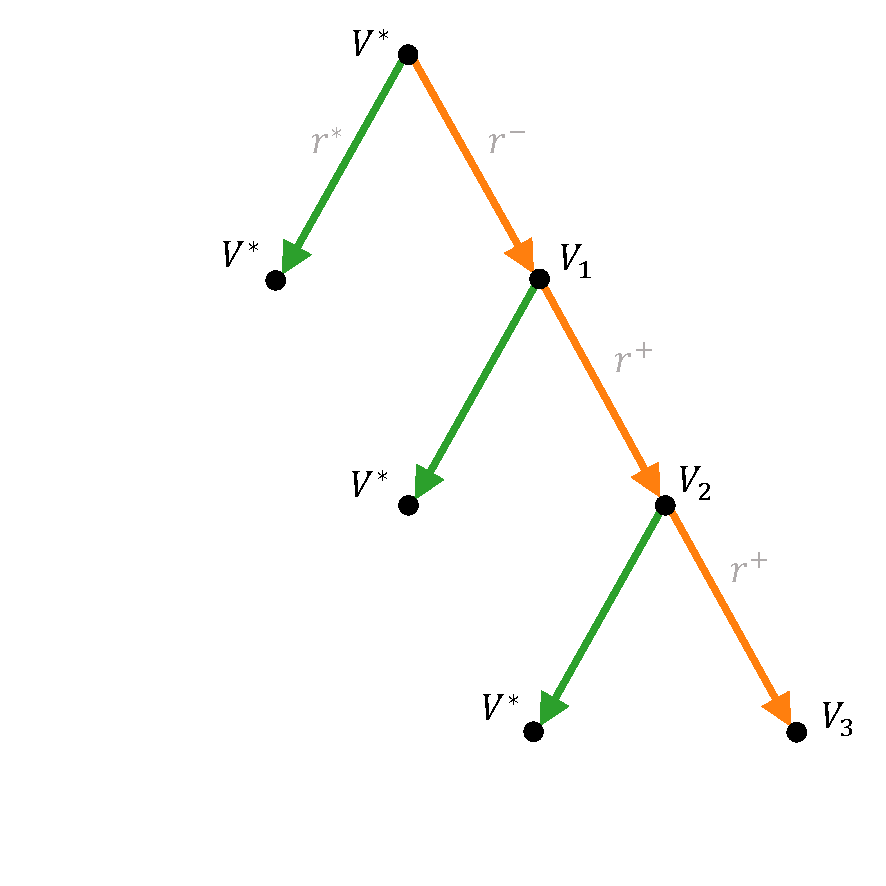
\includegraphics[trim={3.5cm 2cm 0.5cm 0.5cm}, clip, width=0.5\linewidth]{img/gbop/mdp_tree.pdf}
    \caption{Planning tree of the \gls{MDP} $\cM$ of \Cref{fig:mdp}}.
    \label{fig:mdp-tree}
\end{figure}
\begin{lemma}
	\begin{leftbar}[lemmabar]
 Any sequence of actions in $A\setminus{a_1}$ is in $\Tau^\infty$.
 \end{leftbar}
\end{lemma}
\begin{proof}
Any such sequence of actions yields the sequence of rewards $r^-, r^+, \dots,r^+$. and end up in the state $s^+$ with value at least $V^\star$ (obtained by further taking $a_1$ indefinitely). Thus its value $V_h$ verifies, 
\begin{align*}
    V_h &\geq \sum_{t=0}^{h-1} \gamma^t r_t + \gamma^h V^\star\\
    &= r^- - r^+ + \sum_{t=0}^{h-1} \gamma^t r^+ + \gamma^h V^\star \\
    &= (-\frac{\gamma}{1-\gamma} - 1)S + \frac{1-\gamma^h}{1-\gamma} (r^\star + S) + \gamma^h V^\star\\
    &= V^\star - S\frac{\gamma^h}{1-\gamma} \geq V^\star - \frac{\gamma^h}{1-\gamma}
\end{align*}
\end{proof}

We can directly conclude that $\kappa \geq \limsup{|\{a_2,\dots,a_K\}^h|^{1/h}} = K-1$.

Now, consider the nodes expanded by \GBOPD. The first expansion is that of the root, which discovers $s^\star$ and $s^+$. In the absence of information on these two state, the bound $V_{\max}$ is used and the first action $a_1$ gets a higher $\overline{U}$ that any other action $a_2,\dots,a_K$ since $r^\star \geq r^-$. Hence, at the second iteration, the node $a_1$ gets expanded. At this point, the self-loop of the state $s^\star$ is discovered, which means that form now on the bounds verify $L_n(a_1) = V^\star = U_n(a_1)$ for $n\geq2$, which means that $L_n(a_1\cA^*)-U_n(a_1\cA^*) = 0$. The nodes $a_2,\dots,a_K$ can be expanded at most once before the entire \gls{MDP} is discovered and $L_n=V=U_n$ over the entire tree, which means that $\Tau_n^\infty$ is the set of optimal nodes, \ie the nodes in the only optimal sequence $a_1^\star$. Hence, $\kappa_\infty = 1.$ 

\section{Time and memory complexities}

\subsection{\KLOLOP}
\label{sec:kl-olop-time}

After having considered the sample efficiency of \OLOP and \KLOLOP in \Cref{thm:regret-kl-olop}, we now study their time and memory complexities. We will only mention the case of \KLOLOP for ease of presentation, but all results easily extend to \OLOP.

The \Cref{alg:kl-olop} requires, at each episode, to compute and store in memory of the reward upper-bounds and U-values of all nodes in the tree $\Tau = \sum_{h=0}^L \cA^h$.
Hence, its time and memory complexities $C(\KLOLOP)$ are 
\begin{equation*}
C(\KLOLOP) = \cO(M|\Tau|) = \cO(MK^L).
\end{equation*}

The curse of dimensionality brought by the branching factor $K$ and horizon $L$ makes it intractable in practice to actually run \KLOLOP in its original form even for small problems. However, most of this computation and memory usage is wasted, as with reasonable sample budgets $n$ the vast majority of the tree $\Tau$ will not be actually explored and hence does not hold any valuable information.

We propose in \Cref{alg:lazy-kl-olop} a lazy version of \KLOLOP which only stores and processes the explored subtree, as shown in \Cref{fig:tree}, while preserving the inner workings of the original algorithm.

\begin{figure}[ht]
	\centering
	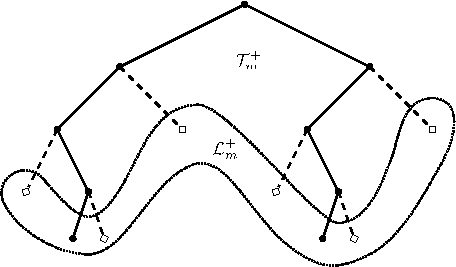
\includegraphics[width=0.6\textwidth]{img/tree_svg-tex}
	\caption{A representation of the tree $\Tau_m^+$, with $K = 2$ actions and after episode $m = 2$, when two sequences have been sampled. They are represented with solid lines and dots \textbullet, and they constitute the explored subtree $\Tau_m$. When extending $\Tau_m$ with the missing children of each node, represented with dashed lines and diamonds $\diamond$, we obtain the full extended subtree $\Tau_m^+$. The set of its leaves is denoted $\LL_m^+$ and shown as a dotted set.}
	\label{fig:tree}
\end{figure}

\begin{algorithm}[tp]
	\DontPrintSemicolon
	Let $M$ be the largest integer such that $M \log M/(2 \log 1/\discount) \leq n$\;
	Let $L = \log M / (2 \log 1/\discount)$\;
	Let $\Tau_0^+ = \LL_0^+ = \{\emptyset\}$\;
	\For{each episode $m = 1, \cdots, M$}{
		Compute $U_a(m-1)$ from \eqref{eq:Ua} for all $a\in\Tau_{m-1}^+$\;
		Compute $B_a(m-1)$ from \eqref{eq:Ba} for all $a\in \LL_{m-1}^+$\;
		Sample a sequence with highest B-value: $a \in \argmax_{a\in \LL_{m-1}^+} B_a(m-1)$\;
		Choose an arbitrary continuation $a^m \in \cA\cA^{L-|a|}$\tcp*{\eg uniformly}
		Let $\Tau_m^+ = \Tau_{m-1}^+$ and $\LL_m^+ = \LL_{m-1}^+$\;
		\For{$t=1, \cdots, L$}{
			\If{$a^m_{1:t} \not \in \Tau_{m}^+$}{
				Add $a^m_{1:t-1}A$ to $\Tau_{m}^+$ and $\LL_{m}^+$\;
				Remove $a^m_{1:t-1}$ from $\LL_{m}^+$
			}
		}
	}
	\Return the most played sequence $a(n) \in \argmax_{a\in \LL_m^+} N_a(m)$
	\caption{Lazy Open Loop Optimistic Planning}
	\label{alg:lazy-kl-olop}
\end{algorithm}


\begin{proposition}[Time and memory complexity]
	\begin{leftbar}[propositionbar]
		\Cref{alg:lazy-kl-olop} has time and memory complexities of
		\begin{equation*}
		C(\texttt{Lazy KL-OLOP}) = O(KLM^2)
		\end{equation*}
		
		The corresponding complexity gain compared to the original \Cref{alg:kl-olop} is: 
		\begin{equation*}
		\frac{C(\texttt{Lazy KL-OLOP})}{C(\KLOLOP)} = \frac{n}{K^{L-1}}
		\end{equation*}
		which highlights that only a subtree corresponding to the sample budget $n$ is processed instead of the search whole tree $\Tau$.
	\end{leftbar}
\end{proposition}
\begin{proof}
	At episode $m = 1, \cdots, M$, we compute and store in memory the reward upper-bounds and U-values of all nodes in the subtree $\Tau_m^+$. Moreover, the tree $\Tau_m^+$ is constructed iteratively by adding K nodes at most L times at each episode from 0 to $m$. Hence, $|\Tau_m^+| = O(mKL)$.
	This yields directly $C(\texttt{Lazy KL-OLOP}) = \sum_{m=1}^M O(mKL) = O(M^2KL)$.
\end{proof}

\begin{proposition}[Consistency]
	\label{prop:consistency}
	\begin{leftbar}[propositionbar]
		The set of sequences returned by \Cref{alg:lazy-kl-olop} is the same as the one returned by \Cref{alg:kl-olop}.
		In particular, \Cref{alg:lazy-kl-olop} enjoys the same regret bounds as in \Cref{thm:regret-kl-olop}.
	\end{leftbar}
\end{proposition}

\begin{proof}
	To prove consistency of \Cref{alg:lazy-kl-olop}, we need to show that the sequences of actions $a^m$ sampled at every episode are chosen arbitrarily from the same sets as in \Cref{alg:lazy-kl-olop}.
	Namely, 
	
	\begin{equation*}
	\left\{ b\in \cA \cA^{L-|a|} : a \in \argmax_{a\in \LL_{m-1}^+} B_a(m-1)\right\} = \argmax_{a\in \cA^L} B_a(m-1)
	\end{equation*}
	
	To that end, we first introduce some useful notations:
	
	\begin{paragraph}{Definition}
		\begin{leftbar}[defnbar]
			% We remind that $\Tau$ refers to the whole search tree $\Tau = \sum_{h=0}^L \cA^h$.
			Let $\Tau_m$ be the set of visited nodes after episode $m$:
			\begin{equation*}
			\Tau_m \eqdef \left\{a\in \cA^*: N_a(m) > 0\right\}
			\end{equation*}
			
			We also define its extension $\Tau_m^+$ of visited nodes and their children:
			\begin{equation*}
			\Tau_m^+ \eqdef \Tau_m + \Tau_m A
			\end{equation*}
			
			Now for $a\in \cA^*$, $\pi_m(a)$ (resp. $\pi_m^+(a)$) refers to its longest prefix within $\Tau_m$ (resp. $\Tau_m^+$):
			\begin{align*}
			\pi_m(a) &\eqdef \argmax_{b\in\Tau_m} \{|b|: a\in b \cA^* \} \\
			\pi_m^+(a) &\eqdef \argmax_{b\in\Tau_m^+} \{|b|: a\in b \cA^* \}
			\end{align*}
			
			Finally, $\LL_m$ and $\LL_m^+$ are the image of $\cA^L$ by $\pi_m$ and $\pi_m^+$, respectively.
			\begin{align*}
			\LL_m &\eqdef \pi_m(\cA^L) \\
			\LL_m^+ &\eqdef \pi_m^+(\cA^L) \}
			\end{align*}
		\end{leftbar}
	\end{paragraph}
	
	\begin{remark}[About children extensions]
		\begin{leftbar}[remarkbar]
			We could frame \Cref{alg:lazy-kl-olop} in terms of $\Tau_m$ and $\LL_m$, for which mathematical proofs are more straight-forward. However, the iterative construction of $\LL_m$ is tricky and it would require inverting $\pi_m$ on $\LL_m$ which is non-trivial. On the contrary, introducing their extensions  $\Tau_m^+$ and $\LL_m^+$ slightly complicates the proof, but greatly simplifies the construction of $\LL_m^+$ and the computation of ${\pi_m^+}^{-1}$ on $\LL_m^+$, which is why we use these sets in practice.
		\end{leftbar}
	\end{remark}
	
	\begin{lemma}[Sets construction]
		\begin{leftbar}[lemmabar]
			$\Tau_m^+$ and $\LL_m^+$ are indeed the sets computed in \Cref{alg:lazy-kl-olop}.
		\end{leftbar}
	\end{lemma}
	\begin{proof}
		Note that for each episode $1 \leq m \leq M - 1$, we have:
		\begin{equation}
		\label{eq:tau_mp1}
		\Tau_{m+1} = \Tau_{m} + \sum_{t=0}^L a^{m+1}_{1:t}
		\end{equation}
		Indeed, the nodes visited at least once at time $m+1$ where either already visited once at time $m$ (\eg in $\Tau_{m}$) or have been visited for the first time during episode $m+1$, which means they are a prefix of $a^{m+1}$. The reverse is clearly true as well.
		
		This enables to write:
		\begin{align*}
		\Tau_{m+1}^+ &= \Tau_{m+1} + \Tau_{m+1}A & \text{by definition}\\
		&= \Tau_{m} + \sum_{t=0}^L a^{m+1}_{1:t} + (\Tau_{m} + \sum_{t=0}^L a^{m+1}_{1:t})A & \text{by \eqref{eq:tau_mp1}} & \\
		&= (\Tau_{m} + \Tau_{m}A) + \sum_{t=0}^L a^{m+1}_{1:t} + \sum_{t=0}^L a^{m+1}_{1:t}A & \\
		&= \Tau_{m}^+ + a^{m+1}_{1:0} + \sum_{t=0}^L a^{m+1}_{1:t}A &\text{ as } \sum_{t=1}^L a^{m+1}_{1:t} \subset \sum_{t=0}^L a^{m+1}_{1:t}A\\
		&=  \Tau_{m}^+ + \sum_{t=0}^L a^{m+1}_{1:t}A  &\text{ as }a^{m+1}_{1:0}=\emptyset \in \Tau_{0} \subset \Tau_{m} \subset \Tau_m^+
		\end{align*}
		This recursion is the one implemented in \Cref{alg:lazy-kl-olop}: at each episode $m$, we add to $\Tau_{m}^+$ the children of the nodes along the sampled action sequence $a^{m}$.
		
		Finally, we highlight that $\LL_m^+ = \pi^+(\cA^L)$ is the set of leaves of $\Tau_{m}^+$.
		Indeed, nodes of $\LL_m^+$ belong to $\Tau_{m}^+$, but they cannot have a child in $\Tau_{m}^+$ as it would contradict the definition of $\LL_m^+$. Conversely, any leaf $a$ of $\Tau_{m}^+$ can be continued arbitrarily to a sequence $b$ of $\cA^L$, which  $a = \pi_m^+(b) \in \pi^+(\cA^L) = \LL_m^+$.
		
		Thus, when updating $\Tau_{m-1}^+$, the set of its leaves is updated accordingly: when the children of a leaf $a^m_{1:t-1}$ are added to $\Tau_m^+$, they become new leaves in place of their parent. Hence, they are added to $\LL_m^+$ while $a^m_{1:t-1}$ is removed from it.
		% 
	\end{proof}
	
	\begin{lemma}[U-values conservation]
		\begin{leftbar}[lemmabar]
			\label{lemma:value-conservation}
			For all $a \in \cA^*$,
			\begin{equation*}
			U_a(m) = U_{\pi_m(a)}(m) = U_{\pi_m^+(a)}(m)
			\end{equation*}
		\end{leftbar}
	\end{lemma}
	\begin{proof}
		Let $a \in \cA^*$, denote $h=|a|$ and $h'=|\pi_m(a)|$.
		
		By definition of $\pi_m(a)$, $0 \leq h' \leq h$, and
		\begin{itemize}
			\item for $1\leq t \leq h'$, we have $a_{1:t} = {\pi_m(a)}_{1:t}$ ;
			\item for $h'+1\leq t \leq h$, we have $a_{1:t} \not \in \Tau_m$, hence $T_{a_{1:t}}(m) = 0$ and $U^{\mu}_{a_{1:t}}(m) = 1$.
		\end{itemize}
		Then,
		\begin{align*}
		U_a(m) &= \sum_{t=1}^h \gamma^t U^{\mu}_{a_{1:t}}(m) + \frac{\gamma^{h+1}}{1-\gamma} \\
		&= \sum_{t=1}^{h'} \gamma^t U^{\mu}_{a_{1:t}}(m) + \sum_{t=h'+1}^h \gamma^t \underbrace{U^{\mu}_{a_{1:t}}(m)}_1 + \frac{\gamma^{h+1}}{1-\gamma} \\
		&= \sum_{t=1}^{h'} \gamma^t U^{\mu}_{{\pi_m(a)}_{1:t}}(m) + \frac{\gamma^{h'+1}}{1-\gamma} \\
		&= U_{\pi_m(a)}(m)
		\end{align*}
		
		Now, consider $\pi_m^+(a) \in \Tau_m^+$.
		By definition, it belongs either to $\Tau_m$ or $\Tau_m A$.
		\begin{itemize}
			\item If $\pi_m^+(a) \in \Tau_m$, then $\pi_m^+(a) = \pi_m(a)$ and $U_{\pi_m^+(a)}(m) = U_{\pi_m(a)}(m)$.
			\item Else, $\pi_m^+(a) \in \Tau_m A$ and $p(\pi_m^+(a)) = \pi_m(a)$.
			
			As $\pi_m^+(a) \not \in \Tau_m$, we have $T_{\pi_m^+(a)}(m) = 0$ and $U^{\mu}_{\pi_m^+(a)}(m) = 1$.
			This yields:
			
			\begin{equation*}
			U_{\pi_m^+(a)}(m) = \sum_{t=1}^{h'} \gamma^t U^{\mu}_{{\pi_m^+(a)}_{1:t}}(m) + \gamma^{h'+1} \underbrace{U^{\mu}_{{\pi_m^+(a)}}(m)}_1 + \frac{\gamma^{h'+2}}{1-\gamma} = U_{\pi_m(a)}(m)
			\end{equation*}
			
		\end{itemize}
		We showed that $U_{\pi_m^+(a)}(m) = U_{\pi_m(a)}(m)$, which concludes the proof.
		% 
	\end{proof}
	
	\begin{lemma}[Inverse projection]
		\begin{leftbar}[lemmabar]
			\label{lemma:inverse-proj}
			For all $a\in \LL_m^+$ of length $h\leq L$,
			\begin{equation*}
			{\pi_m^+}^{-1}(a) = a \cA^{L-h}
			\end{equation*}
			
			This allows to easily pick a sequence inside ${\pi_m^+}^{-1}(a)$: just continue the sequence $a$ with a default action of $A$ (\eg the first) until it reaches length $L$.
		\end{leftbar}
	\end{lemma}
	\begin{proof}
		Let $a\in \LL_m^+$. 
		
		By definition of $\pi_m^+$, any sequence in ${\pi_m^+}^{-1}(a)$ is a suffix of $a$ of length $L$, so we clearly have the direct inclusion ${\pi_m^+}^{-1}(a) \subset a \cA^{L-h}$.
		
		Now for the other side: let $b\in \cA \cA^{L-h}$, \ie $a=b_{1:h}$. We need to show that $\pi_m^+(b) = a$.
		As $a\in \LL_m^+$, there exists $c\in \cA^L$ such that $\pi_m^+(c) = a$.
		\begin{itemize}
			\item If h = L, then $b=a$, so $b \in \LL_m^+ \subset \Tau_m^+$, and hence $\pi_m^+(b)=b=a$.
			\item If h < L, we can show by contradiction that $a \not \in \Tau_m$. Indeed, if $a \in \Tau_m$, then $c_{1:h+1}$ is the child of a node of $\Tau_m$ and hence belongs to $\Tau_m^+$. But then, $c_{1:h+1}$ is a prefix of $c$ in $\Tau_m^+$ with greater length than $a$, which contradicts the definition of $a = \pi_m^+(c)$.
			
			Now, because $a \not \in \Tau_m$, it is also true for all suffixes of $a$, and in particular for $b_{1:t}$ with $h \leq t \leq L$. Indeed, we have $a^s_{1:t} = b_{1:t} \implies a^s_{1:h} = b_{1:h} = a$, so:
			\begin{equation*}
			T_{b_{1:t}}(m) = \sum_{s=1}^m \mathbbm{1}\{a^s_{1:t} = b_{1:t}\} \leq \sum_{s=1}^m \mathbbm{1}\{a^s_{1:h} = a\} = N_a(m) = 0
			\end{equation*}
			Hence, $b_{1:t} \not \in \Tau_m$ for all $h \leq t \leq L$, so in particular $b_{1:t} \not \in \Tau_m^+$ for all $h+1 \leq t \leq L$. Since $b_{1:h} = a \in \Tau_m^+$, $a$ is indeed the longest prefix of $b$ in $\Tau_m^+$, that is: $\pi_m^+(b) = a$.
		\end{itemize}
		We have shown the other side of the inclusion: $a \cA^{L-h} \subset {\pi_m^+}^{-1}(a)$, which entails that the two sets are in fact equal.
		% 
	\end{proof}
	
	We can now conclude our proof of \Cref{prop:consistency}: at episode $m$, \KLOLOP samples a sequence of action $a^m$ within the set $\argmax_{a\in \cA^L} U_a(m)$. 
	However, we have:
	
	\begin{align*}
	\argmax_{c\in \cA^L} U_c(m) &= \argmax_{c\in \cA^L} U_{\pi_m^+(c)}(m) & \text{by \Cref{lemma:value-conservation}} \\
	&= {\pi_m^+}^{-1}\left(\argmax_{a\in {\pi_m^+}(\cA^L)} U_{a}(m)\right) & \\
	&= \left\{b\in{\pi_m^+}^{-1}(a) : a\in \argmax_{a\in \LL_m^+} U_{a}(m)\right\} & \\
	&= \left\{b\in \cA \cA^{L-|a|} : a\in \argmax_{a\in \LL_m^+} U_{a}(m)\right\} & \text{by \Cref{lemma:inverse-proj}} 
	\end{align*}
	
	Thus, at each episode the sequence of actions $a^m$ sampled by \Cref{alg:lazy-kl-olop} could have been sampled by \Cref{alg:kl-olop} as well.
	
	In particular, if the arbitrary rule used to pick a sequence from a set is the same for the two algorithms, then the sampled sequences $a^m$ will be identical, will have the same visit count $T_{a^m}(m)$, and in the end the returned action $a(n)$ will be the same.
	% 
\end{proof}

\subsection{\GBOP}
\label{sec:gbop-implementation}

In this section, we provide more details about the implementation of \GBOPD and \GBOP. First, we discuss how two procedures can be approximated so that they terminate in finite time, and study the impact of this approximation on the regret guarantees. Second, we propose a lazy implementation of the bounds computation through $\cB_n^\infty$ that only considers a subset of nodes to update.

\subsubsection{Termination}

\paragraph{Bounds computation}

The bounds computation step $\cB_n^\infty$ (line 1 of \GBOPD) can converge in infinite time whenever $\cG_n$ contains a loop, as shown in \Cref{fig:simple_loop}. We consider the effect of stopping early after a fixed number of iterations $k(\varepsilon,\gamma)$.

\begin{figure}[th]
	\centering
	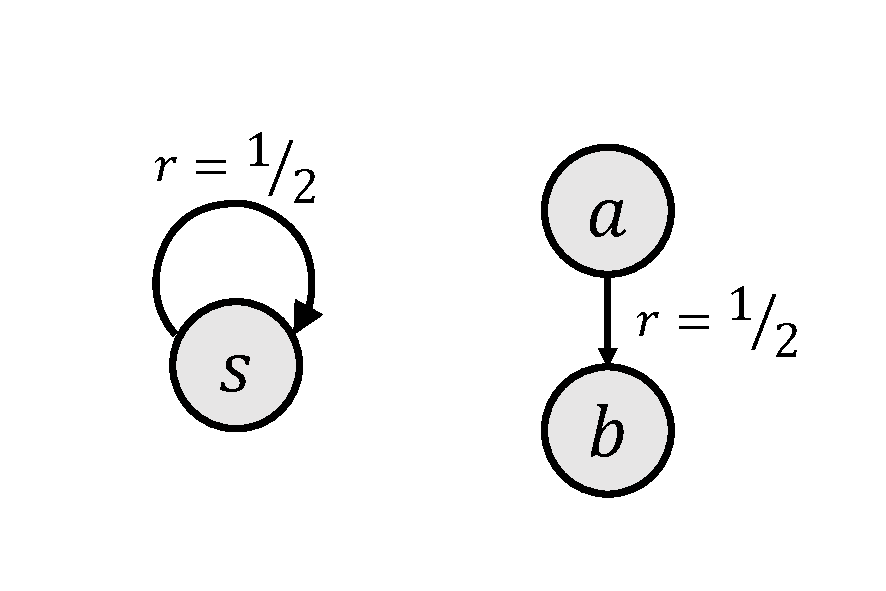
\includegraphics[trim=2.5cm 1cm 9cm 2cm, clip, width=0.1\linewidth]{img/gbop/loop.pdf}\\
	\begin{tabular}{lccccc}
		\toprule
		$k$ & $0$ & $1$ & $\cdots$ & $k$ \\
		\midrule
		$\cU = \cB^k(V_{\max})(s)$ & $V_{\max}$ & $\frac{1}{2} + \gamma V_{\max}$ && $\frac{1}{2}(1-\gamma^k)V_{\max} + \gamma^k V_{\max}$\\
		$\cL = \cB^k(0)(s)$ & $0$ & $\frac{1}{2}$ && $\frac{1}{2}(1-\gamma^k)V_{\max}$\\
		\bottomrule
	\end{tabular}
	\caption{\textbf{Top}: a simple looping MDP with $|S|=|A|=1$ after having observed a single transition ($n=1$). \textbf{Bottom}: the sequence of bounds $\cB_1^k(0)$ and $\cB_1^k(V_{\max})$. They converge geometrically to their limit $\cU_1 = \cL_1 = V = \frac{1}{2}V_{\max}$, thus in infinite time.}
	\label{fig:simple_loop}
\end{figure}

\begin{proposition}[Time complexity of bounds computation]
	\begin{leftbar}[propositionbar]
		An $\varepsilon$-approximation of $(\cL_n, \cU_n)$ can be computed by applying $\cB_n$ for a finite number $k(\epsilon,\gamma)$ of iterations, with $$k(\epsilon,\gamma) = \log_\gamma\frac{1}{\varepsilon(1-\gamma)}.$$ 
	\end{leftbar}
\end{proposition}
\begin{proof}
	$\cB_n$ is a $\gamma$-contraction by \Cref{lem:properties-b-graph}, and $\cU_n$ (resp $\cL_n$) is at a distance (in $\|\dot\|_\infty$) at most $V_{\max}$ of the initial value bound $V_{\max}$ (resp $0$). Thus, the $k^{\text{th}}$ application of $\cB_n$ decreases this error by a factor $\gamma^k$, which gives the result.
\end{proof}

The impact of using an $\varepsilon$-approximation of $(\cL_n, \cU_n)$ during planning is the following:
\begin{proposition}[Effect of early stopping]
	\begin{leftbar}[propositionbar]
		\label{prop:early-stopping}
		Denote the approximate bounds $(\hat{\cL}_n, \hat{\cU}_n)$ obtained by applying $\cB_n^{k(\varepsilon,\gamma)}$ instead of $\cB_n^\infty$, and likewise $(\hat{L}_n, \hat{U}_n)$ in their tree version obtained by applying $B_n^{k(\varepsilon,\gamma)}$ instead of $B_n^\infty$.
		Then, running \GBOPD with $\hat{\cL}_n, \hat{\cU}_n$ gives the following regret:
		\begin{align*}
		\regret = \tilde{\cO}\left(n^{-\log \frac{1}{\gamma}/\hlob{\log \hat{\kappa}_\infty}}\right),
		\end{align*}
		with $$\hlgb{{\kappa}_\infty} \leq \hlob{\hat{\kappa}_\infty \eqdef \lim_{n\rightarrow\infty} \kappa(\hat{L}_n, \hat{U}_n)} \leq \hlrb{\kappa}.$$
		Moreover, the approximation gap $\hlgb{\kappa_\infty} - \hlob{\hat{\kappa}_\infty}$ is non-increasing with respect to $\varepsilon$.
	\end{leftbar}
\end{proposition}
It is difficult to control more explicitly the gap between $\hlgb{\kappa_\infty}$ and $\hlob{\hat{\kappa}_\infty}$, which might be discontinuous with $\varepsilon$.

\begin{proof}
	Note that $\hat{L}_n$ and $\hat{U}_n$ are valid monotonic bounds on $V$, verifying
	\[0\leq \hat{L}_n\leq {L}_n \leq V \leq {U}_n\leq \hat{U}_n \leq V_{\max}.\]
	Thus, \Cref{lem:bounds} holds with the difference that we only have an inequality $$\overline{U_n}(a) \geq \max_{a'\in a \cA^\infty} \overline{U}(a')$$ rather than an equality, by monotonicity but non-invariance by $B_n$. However, this was the actual inequality used in \Cref{lem:expansion-bound}, which still holds by replacing $L_n,U_n$ by their approximation $\hat{L}_n,\hat{U}_n$. Likewise, \Cref{lem:recommendation-bound} holds. The proof of \Cref{thm:regret-gbop}, can be written with the modification that expanded nodes belong to $T_h^\infty(\hat{L}_n, \hat{U}_n))$, which gives the claimed bound.
	
	As $\varepsilon$ decreases, $k(\epsilon,\gamma)$ increases, which means by \Cref{lem:properties-b-tree} that $(\hat{\cL}_n, \hat{\cU}_n)$ get tighter and $\hlob{\hat{\kappa}_\infty}$ shrinks by \Cref{lem:shrink}. It reaches its minimum $\hlgb{\kappa_\infty}$ when $\varepsilon=0$.
\end{proof}

Thus, we observe that there is a \emph{tradeoff} between the time complexity $k(\varepsilon)$ and the sample complexity $\hlob{\hat{\kappa}_\infty}$: decreasing one increases the other.

Note that \OPD uses $d_n$ iterations of $B_n$, which corresponds to a tuning of $\varepsilon$ with $n$: $\varepsilon_n = \frac{\gamma^{d_n}}{1-\gamma} = \cO(n^{-\frac{\log 1/\gamma}{\log \kappa}})$. 


\paragraph{Sampling rule}

The sampling rule of \GBOPD (line 2 of \GBOPD) can yield an infinite sequence $b_n$. We propose to stop the sampling after a fixed depth $d^+_n$.

\begin{proposition}[Time complexity of sampling]
	\begin{leftbar}[propositionbar]
		Consider the variant of \GBOPD where we stop the sampling rule when reaching a fixed depth $d^+_n$ chosen polynomial with $n$:
		\[d^+_n = \ceil{\alpha n^\beta},\; \text{with }\alpha,\beta > 0\]
		Then, the regret bound of \Cref{thm:regret-gbop} (or that of \Cref{prop:early-stopping} when using early stopping in the bounds computation) still holds.
	\end{leftbar}
\end{proposition}

Note that this is not too constraining compared to \OPD, for which the sampling rule complexity $d_n$ is upper-bounded by $n$. Hence, by choosing $\alpha=\beta=1$, \GBOPD preserve the same complexity as \OPD in the worst case.

\begin{proof}
	Let $\kappa'>\hlgb{{\kappa}_\infty}$ (or $\kappa'>\hlob{\hat{\kappa}_\infty}$ under approximate bounds). In the proof of \Cref{thm:regret-gbop}, it is shown that the maximum depth $d_n$ of an expanded node is at least $d^-_n \eqdef \log_{\kappa'}\frac{n-C_0}{C_1'}$, which allows to conclude with \Cref{lem:recommendation-bound} that $\regret = \cO(\gamma^{d_n}) = \cO(\gamma^{d^-_n})$. By choosing $d^+_n$ polynomial, we have that $d^+_n$ is greater than $d^-_n$ for $n$ sufficiently high. Thus, by stopping the sampling after reaching a depth $d^+_n$, we have that $\regret \leq \gamma^{\min\{d_n, d^+_n\}} / (1-\gamma) = \cO(\gamma^{d^-_n}) = \cO(n^{\frac{-\log 1/\gamma}{\log \kappa'}})$
\end{proof}

\subsubsection{Efficient implementation of $\cB_n^\infty$}

The bounds $\cL_n$ and $\cU_n$ are computed by fixed-point iteration of $\cB_n$ from the trivial bounds $(0,V_{\max})$. The naive implementation of $\cB_n$ requires to iterate over the whole set of state-action pairs in $\cG_n$. 
Two ideas can be used to increase the efficiency of both steps:
\begin{enumerate}[label=(\roman*)]
	\item Instead of starting the iteration with the trivial bounds, the previous estimate $\cL_{n-1}, \cU_{n-1}$ can be used instead at iteration $n$. Since these bounds are closer to their limit ($0\leq \cL_{n-1}\leq \cL_n$ and $\cU_n\leq \cU_{n-1} \leq V_{\max}$), the fixed-point iteration will converge quicker.
	\item In particular, since $\cL_{n-1}$ and $\cU_{n-1}$ are invariant by $\cB_n$, the the only nodes modified by a supplementary application of $\cB_n$ are the parents of only updated node: the expanded state $s_n$. Once its value is updated by $\cB_n$, the same reasoning can be applied for the next iteration of $\cB_n$: only its predecessors can be updated. Thus, we can keep track of a set $q$ of states that can be updated, for every application of $\cB_n$.
\end{enumerate}
These idea are formalised in \Cref{alg:queue-b-inf}. Note that the criterion $\|\cB_n^{k+1} - \cB_n^k\| \leq \frac{1-\gamma}{\gamma}\varepsilon$ is used to detect that the limit $\cB_n^\infty$ is approximated with accuracy $\varepsilon$, and stems from $\cB_n$ being a $\gamma$-contraction:
\begin{proof}
	$\|\cB_n^k - \cB_n^\infty\| \leq \gamma\| \cB_n^{k+1} - \cB_n^\infty\| \leq \gamma \|\cB_n^{k+1} - \cB_n^{k}\| + \gamma \|\cB_n^{k} - \cB_n^\infty\|$, with $\| \cB_n^{k+1} - \cB_n^{k}\| \leq \frac{1-\gamma}{\gamma}\varepsilon$, thus $\|\cB_n^{k} - \cB_n^\infty\| \leq \varepsilon$.
\end{proof}

\begin{algorithm}
	\caption{A queue-based implementation of $\cB_n^\infty$.}
	\label{alg:queue-b-inf}
	\KwIn{Initial bound $\cU_{n-1}$, expanded node $s_n$, accuracy $\varepsilon$}
	\KwOut{An $\varepsilon$-approximation of $\cU_{n}$}
	\DontPrintSemicolon
	$\cU_n \gets \cU_{n-1}$\;
	$q\gets [s_n]$\;
	\While{$q$ is not empty}{
		$s'\gets$ Pop the first node from the queue $q$\;
		$\cU' \gets \cB_n(\cU_n)(s')$\Comment*[r]{Node backup}
		\If(\Comment*[f]{Stopping rule}){$\cU' - \cU_n > \frac{1-\gamma}{\gamma}\varepsilon$}{
			Push the predecessors $s$ of $s'$ to the queue $q$ \Comment*[r]{Propagation rule}
		}
		$\cU_n(s') \gets \cU'$\;
	}
	\Return $\cU_n$\;
\end{algorithm}

